\subsection*{1. Ephemeral versus Persistent (Regular) znodes}
\addcontentsline{toc}{section}{1. Ephemeral versus Persistent (Regular) znodes}

\subsubsection{1.1 - Inicialize a interface de comando de linha (CLI): bin/zkCli.sh
-server 127.0.0.1:2181}
\addcontentsline{toc}{subsection}{1.1 Inicialize o CLI}

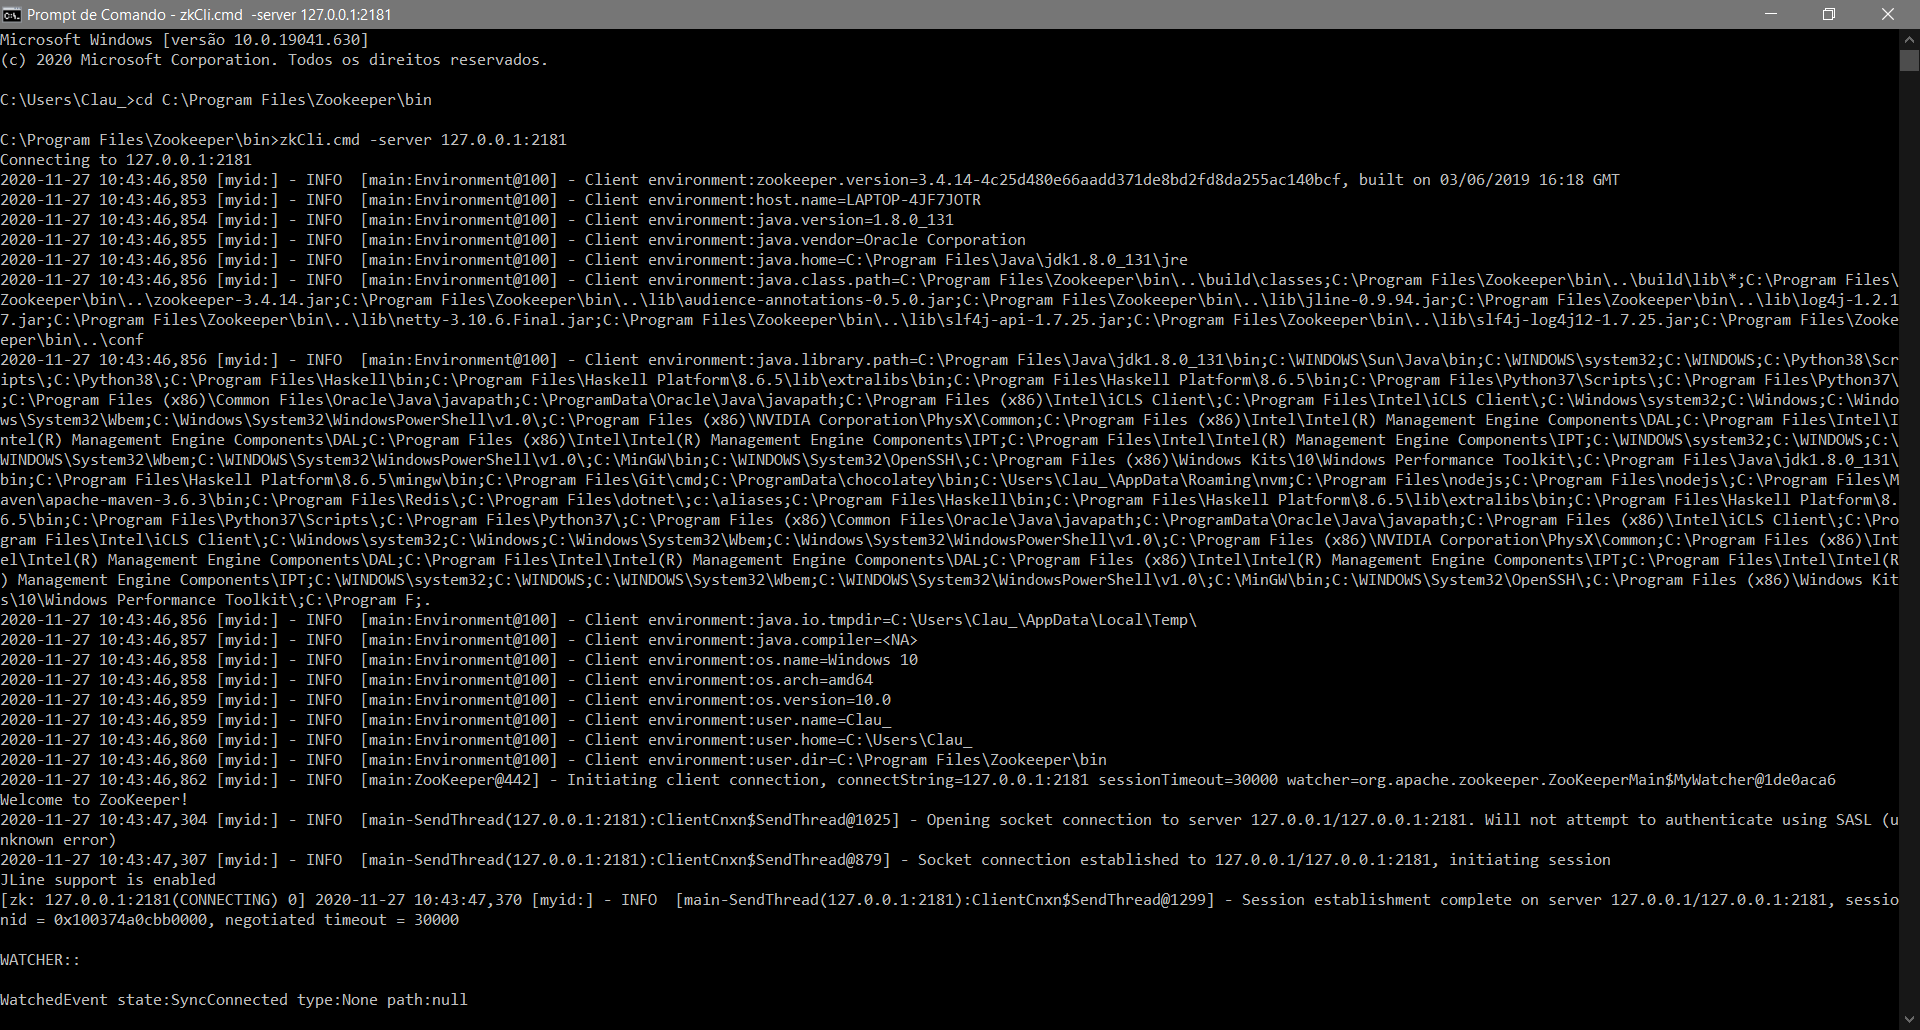
\includegraphics[width=20cm]{pratica3/prints/client1_started.PNG}

\subsubsection{1.2 - Crie um znode persistente para este exercício: create /mcta025 data}
\addcontentsline{toc}{subsection}{1.2 Crie um znode persistente para este exercício}

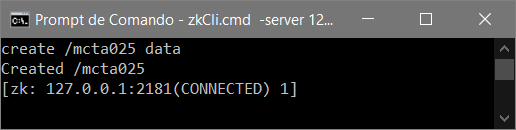
\includegraphics{pratica3/prints/roteiro 1.2.PNG}

\subsubsection{1.3 - Crie um outro znode persistente: create /mcta025/ex1 data}
\addcontentsline{toc}{subsection}{1.3 Crie um outro znode persistente}

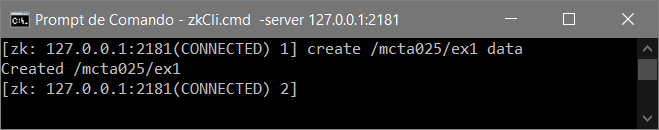
\includegraphics{pratica3/prints/roteiro 1.3.PNG}

\subsubsection{1.4 - Crie um znode efêmero: create -e /mcta025/ex1/ephemeral data}
\addcontentsline{toc}{subsection}{1.4 Crie um znode efêmero}

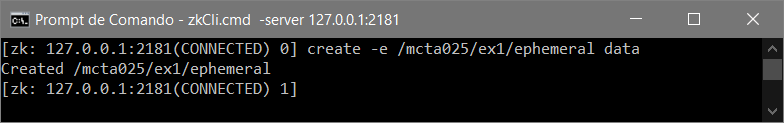
\includegraphics{pratica3/prints/roteiro 1.4.PNG}

\subsubsection{1.5 - Liste os filhos do seu sistema de arquivo (na API, getChildren): ls
<path>}
\addcontentsline{toc}{subsection}{1.5 Liste os filhos do seu sistema de arquivo}

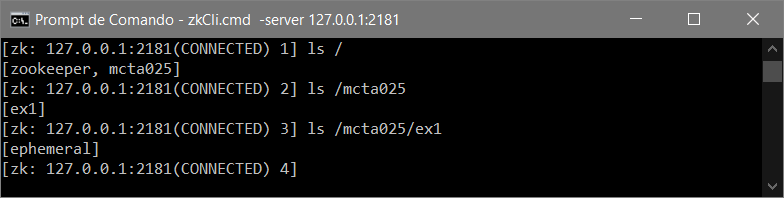
\includegraphics{pratica3/prints/roteiro 1.5.PNG}

\subsubsection{1.6 - Saia do cliente usando o comando quit}
\addcontentsline{toc}{subsection}{1.6 Saia do cliente usando o comando quit}

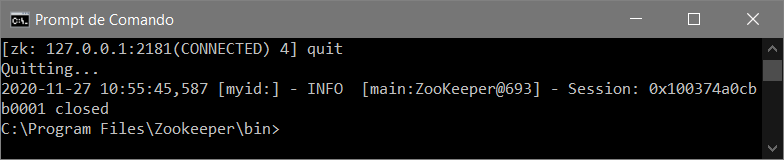
\includegraphics{pratica3/prints/roteiro 1.6.PNG}

\subsubsection{1.7 - Reinicie a CLI e liste novamente os filhos do sistema de arquivo. O que aconteceu?}
\addcontentsline{toc}{subsection}{1.7 Reinicie a CLI e liste novamente os filhos do sistema de arquivo}

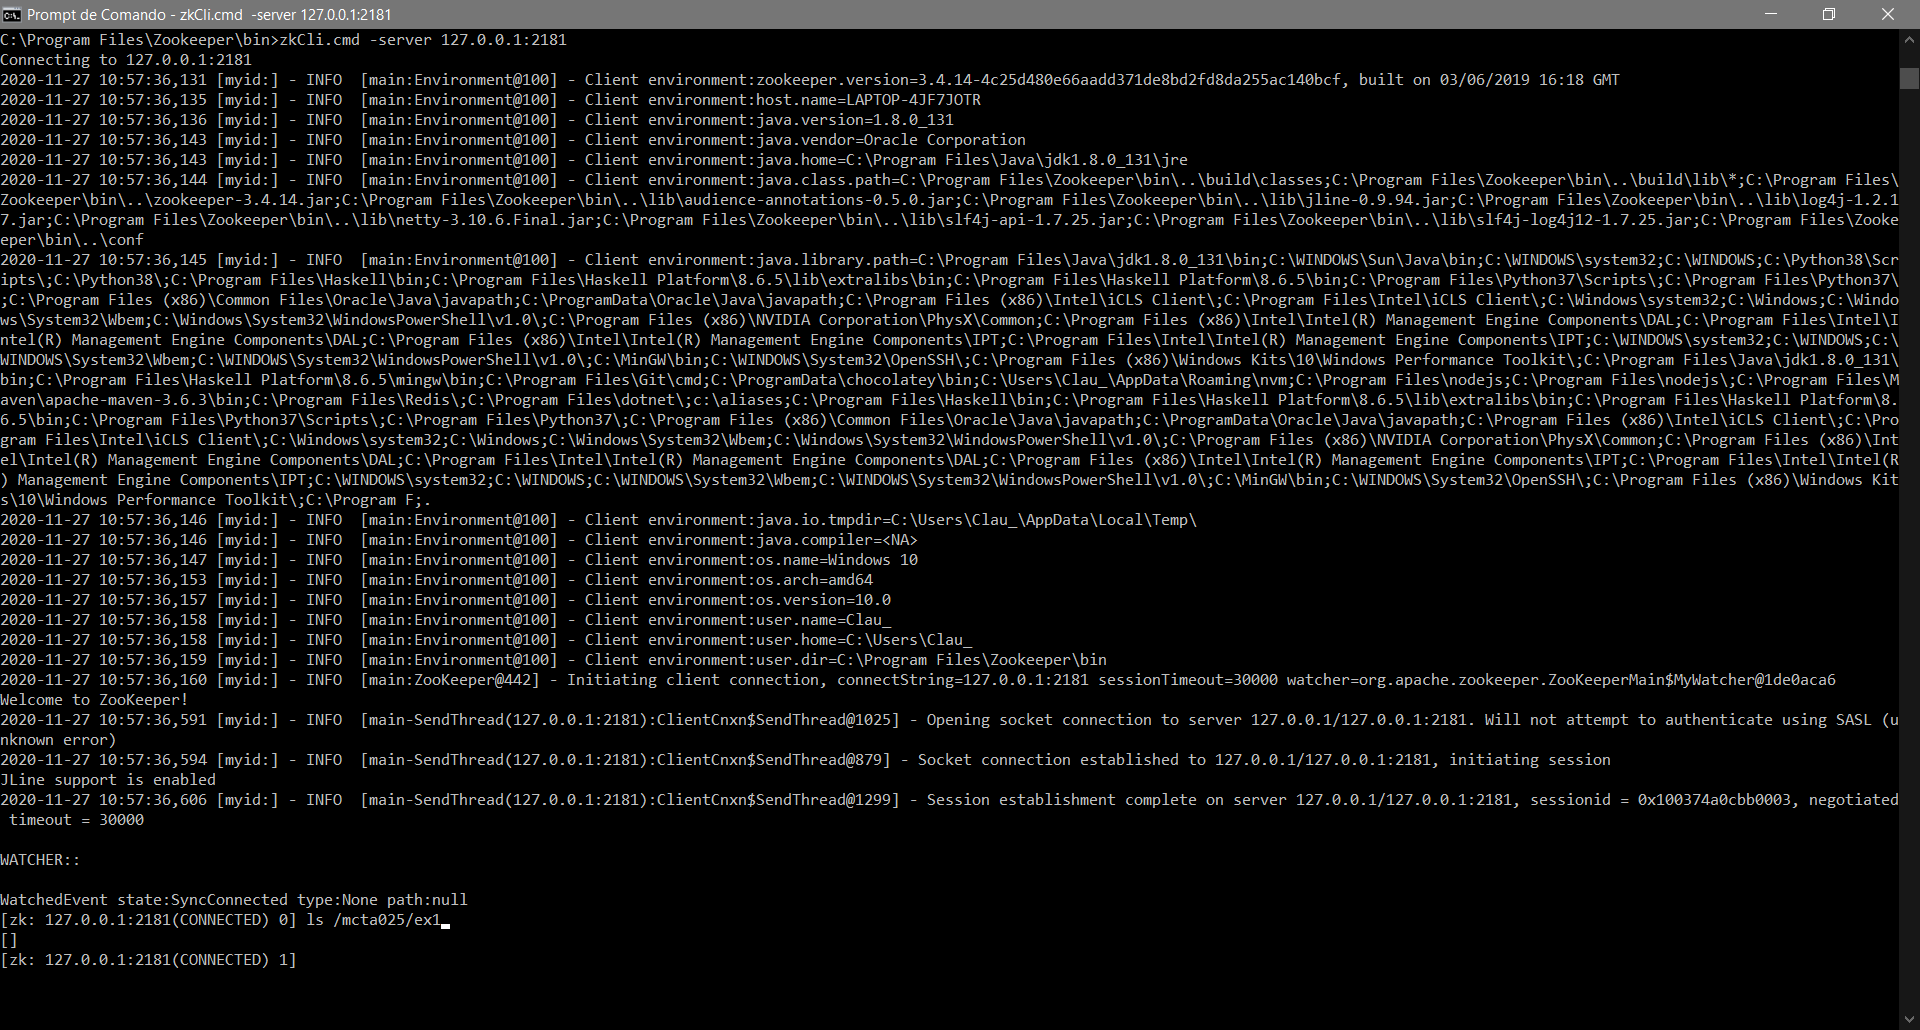
\includegraphics[width=20cm]{pratica3/prints/roteiro 1.7.PNG}

\subsubsection{1.8 - Crie um novo znode efêmero: create -e /mcta025/ex1/ephemeral1 data. Então, crie um filho para o znode que acabou de ser criado: create /mcta025/ex1/ephemeral1/child data. O que aconteceu?}
\addcontentsline{toc}{subsection}{1.8  Tente criar um filho de um znode efêmero}

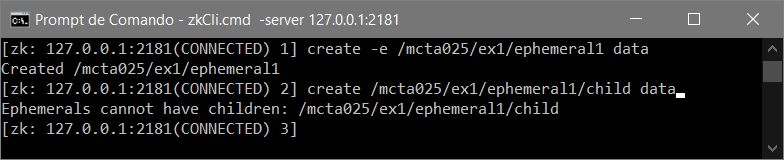
\includegraphics{pratica3/prints/roteiro 1.8.PNG}

\subsection*{2. Sequential suffix}
\addcontentsline{toc}{section}{2. Sequential suffix}

\subsubsection{2.1 - Crie um outro znode persistente: create /mcta025/ex2 data}
\addcontentsline{toc}{subsection}{2.1  Crie um outro znode persistente}

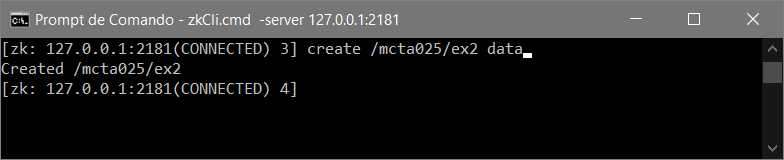
\includegraphics{pratica3/prints/roteiro 2.1.PNG}

\subsubsection{2.2 - Crie znodes sequenciais (com sufixo sequencial): create -s
/mcta025/ex2/child data. Repita o comando várias vezes. Qual o
comprimento do sufixo?}
\addcontentsline{toc}{subsection}{2.2  Crie znodes sequenciais}

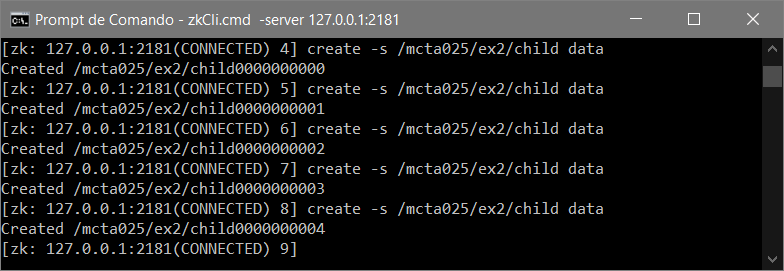
\includegraphics{pratica3/prints/roteiro 2.2.PNG}

\subsubsection{2.3 - Crie znodes sequenciais efêmeros: create -s -e
/mcta025/ex2/child data. Repita o comando várias vezes}
\addcontentsline{toc}{subsection}{2.3 Crie znodes sequenciais efêmeros}

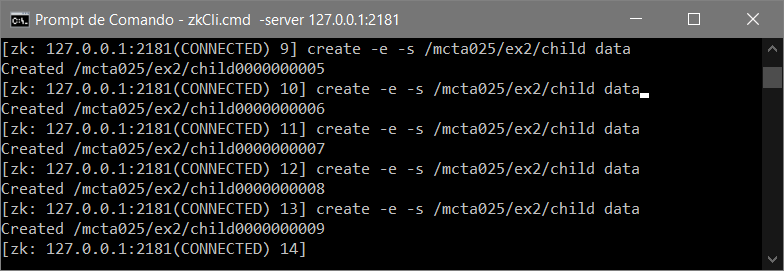
\includegraphics{pratica3/prints/roteiro 2.3.PNG}

\subsubsection{2.4 - Remova alguns znodes com o comando: delete <path>.}
\addcontentsline{toc}{subsection}{2.4   Remova alguns znodes}

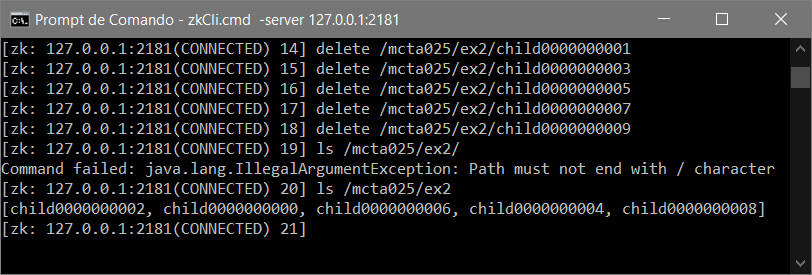
\includegraphics{pratica3/prints/roteiro 2.4.PNG}

\subsubsection{2.5 - Crie mais alguns znodes sequenciais. Como fica a numeração deles?}
\addcontentsline{toc}{subsection}{2.5  Crie mais alguns znodes sequenciais}

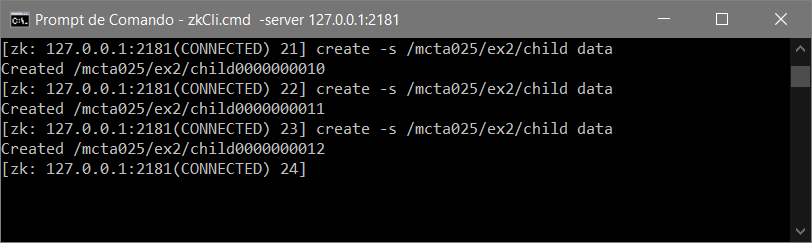
\includegraphics{pratica3/prints/roteiro 2.5.PNG}

\subsubsection{2.6 - Crie znodes sequenciais com outro prefixo: create -s
/mcta025/ex2/son data. Como fica a numeração deles?}
\addcontentsline{toc}{subsection}{2.6  Crie znodes sequenciais com outro prefixo}

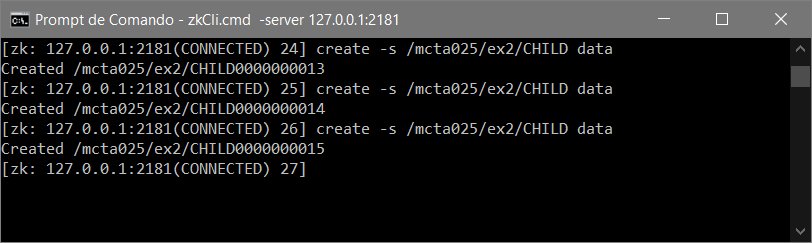
\includegraphics{pratica3/prints/roteiro 2.6.PNG}

\subsubsection{2.7 - Crie outros znodes sequenciais em /mcta025. A numeração (isto é, o escopo) está relacionada com a numeração anterior?}
\addcontentsline{toc}{subsection}{2.7 Crie outros znodes sequenciais e correlacione com a numeração anterior}

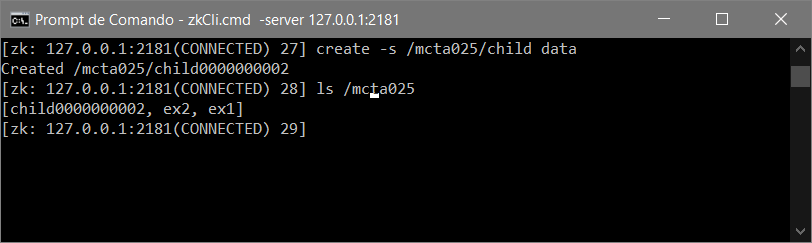
\includegraphics{pratica3/prints/roteiro 2.7.PNG}


\subsection*{3. Watches}
\addcontentsline{toc}{section}{3. Watches}

\subsubsection{3.1 - Todas as operaçõs de leitura no ZooKeeper tem a opção de se
configurar um watch. Abra um segundo cliente em paralelo, que
chamaremos de Cliente 2. O cliente inicial será chamado de Cliente 1.}
\addcontentsline{toc}{subsection}{3.1 Abra um segundo cliente em paralelo}

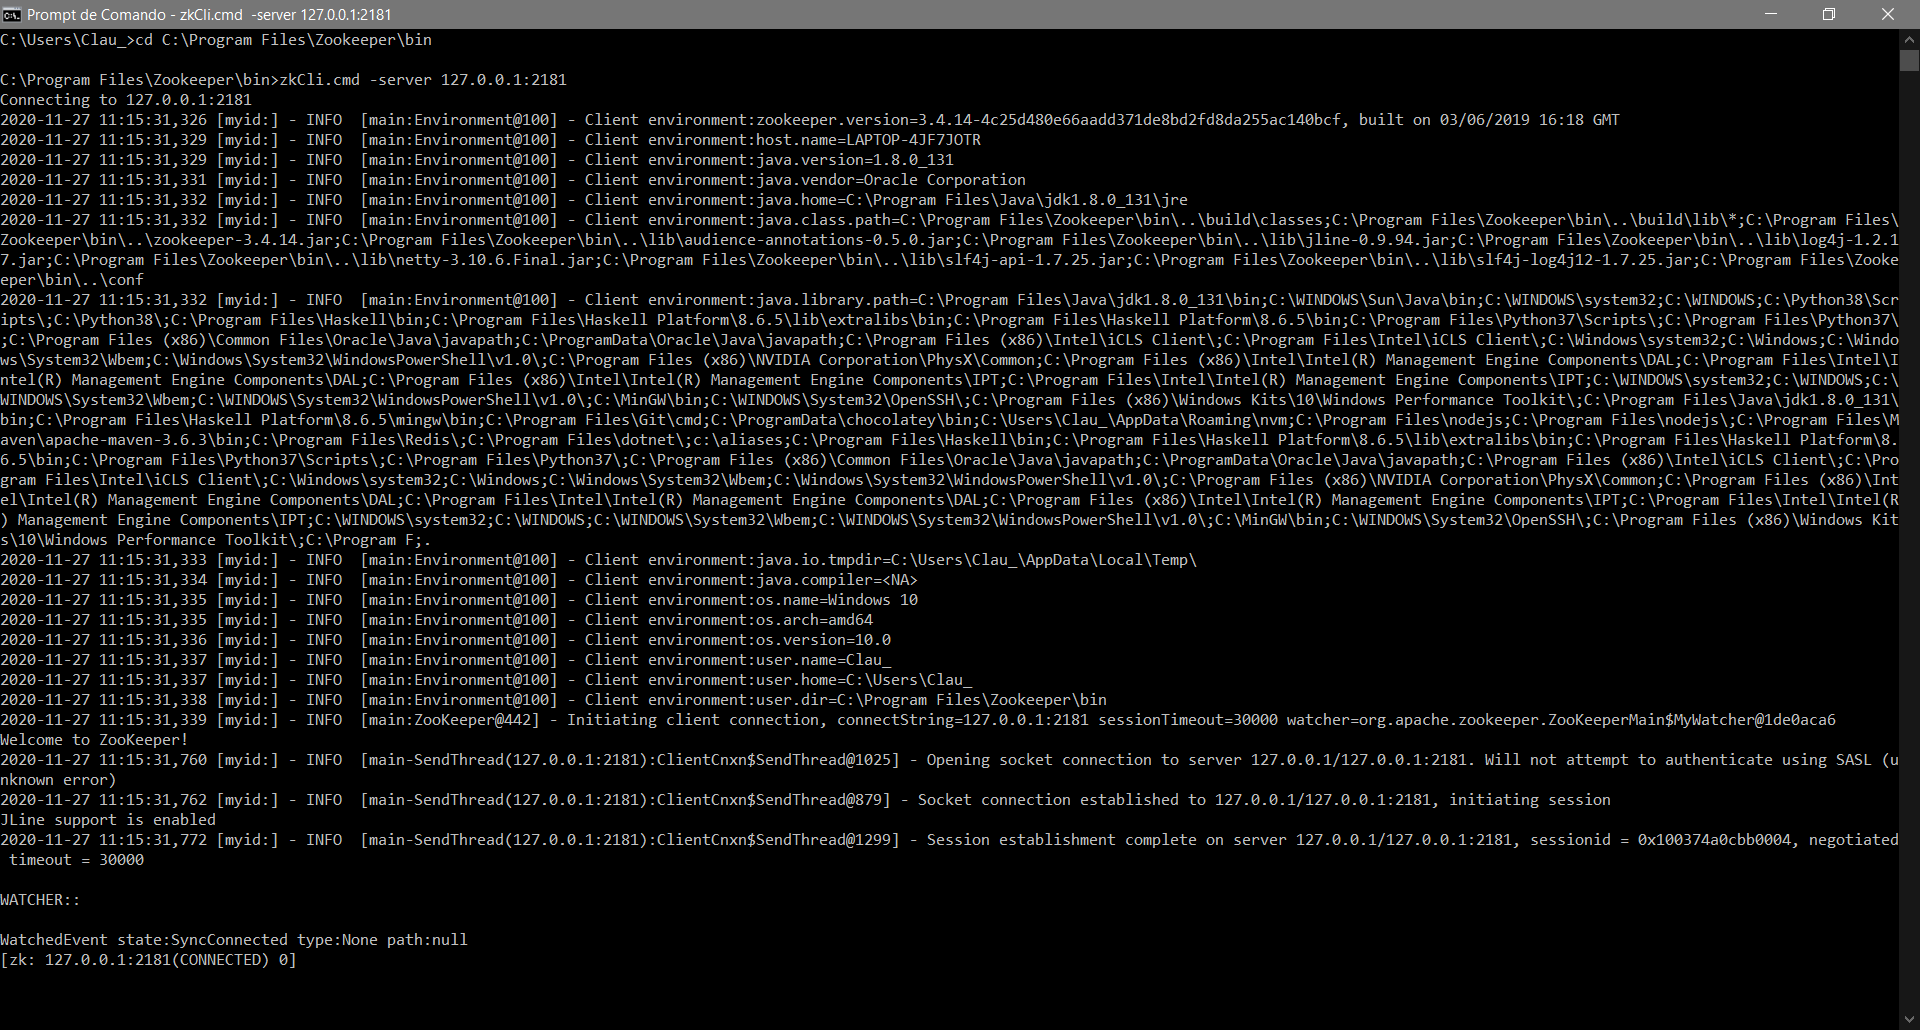
\includegraphics[width=20cm]{pratica3/prints/client2_started.PNG}

\subsubsection{3.2 - Crie um novo znode através do Cliente 1: create /mcta025/ex3
data.}
\addcontentsline{toc}{subsection}{3.2 Crie um novo znode através do Cliente 1}

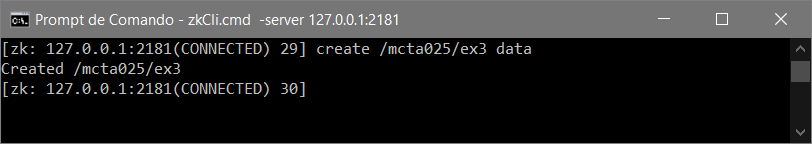
\includegraphics{pratica3/prints/roteiro 3.2.PNG}

\subsubsection{3.3 - Configure um watch de dados do nó que acabou de ser criado no
Cliente 1: get /mcta025/ex3 true}
\addcontentsline{toc}{subsection}{3.3 Configure um watch de dados do nó que acabou de ser criado no Cliente 1}

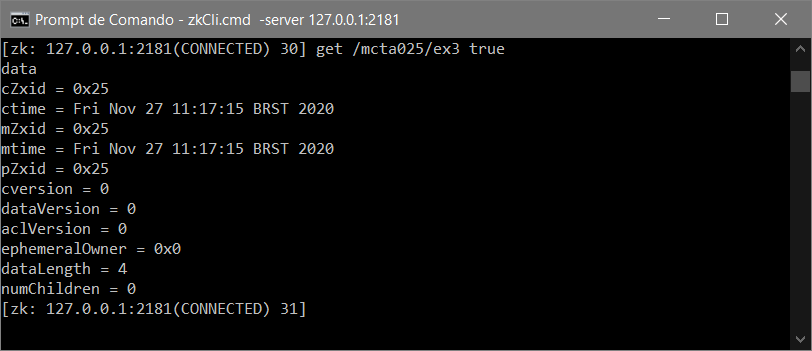
\includegraphics{pratica3/prints/roteiro 3.3.PNG}

\subsubsection{3.4 - No Cliente 2, modifique os dados do nó: set /mcta025/ex3
newData. O que acontece no Cliente 1?}
\addcontentsline{toc}{subsection}{3.4  Modifique os dados do nó no cliente 2}

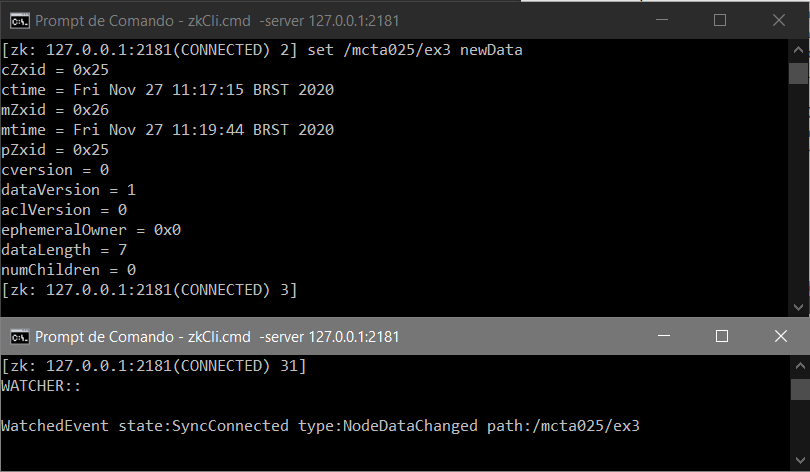
\includegraphics{pratica3/prints/roteiro 3.4.PNG}

\subsubsection{3.5 - Repita no Cliente 2 o comando anterior. O que aconteceu no Cliente 1? Justifique.}
\addcontentsline{toc}{subsection}{3.5 Repita no Cliente 2 o comando anterior}

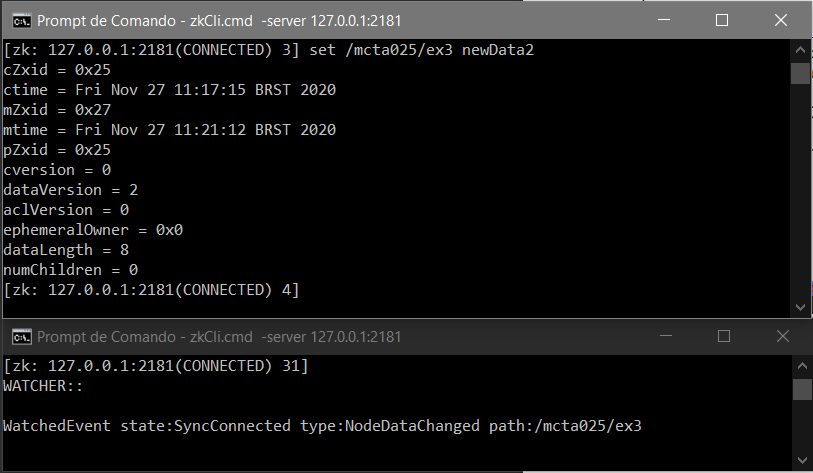
\includegraphics{pratica3/prints/roteiro 3.5.PNG}

\subsubsection{3.6 - É possível instalar watch de filhos de um nó. No Cliente 1: ls
/mcta025/ex3 true. Então, no Cliente 2, crie um novo filho dentro de /mcta025/ex3. O que aconteceu?}
\addcontentsline{toc}{subsection}{3.6 ?}

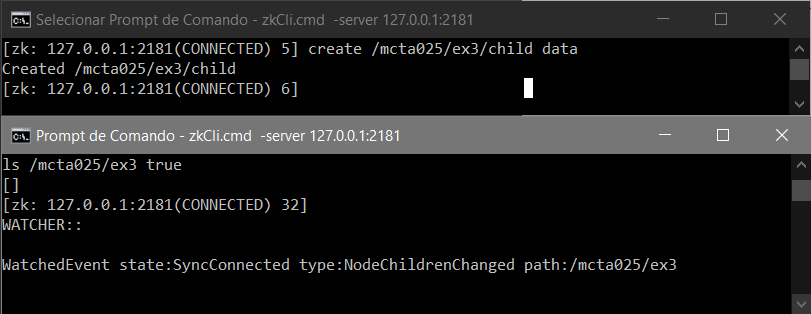
\includegraphics{pratica3/prints/roteiro 3.6.PNG}

\subsubsection{3.7 - Crie um watch de dados para /mcta025/ex3. No Cliente 2, crie um
filho em /mcta025/ex3. O que aconteceu? Justifique.}
\addcontentsline{toc}{subsection}{3.7 ?}

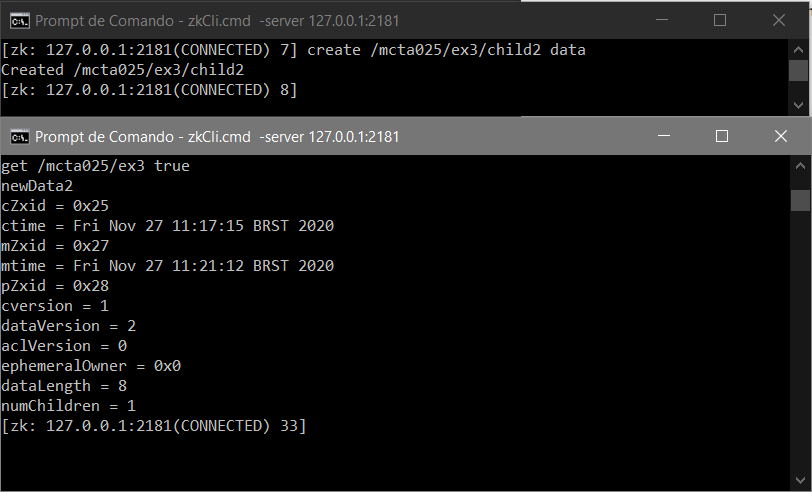
\includegraphics{pratica3/prints/roteiro 3.7.PNG}

\subsubsection{3.8 - Crie um watch de filhos para o nó /mcta025/ex3 e um watch de filhos para um filho dele usando o Cliente 1. No Cliente 2, crie um filho no
nó filho criado anteriormente. O que aconteceu? Agora crie um filho
em /mcta025/ex3. O que podemos concluir dessas operações?}
\addcontentsline{toc}{subsection}{3.8 ?}

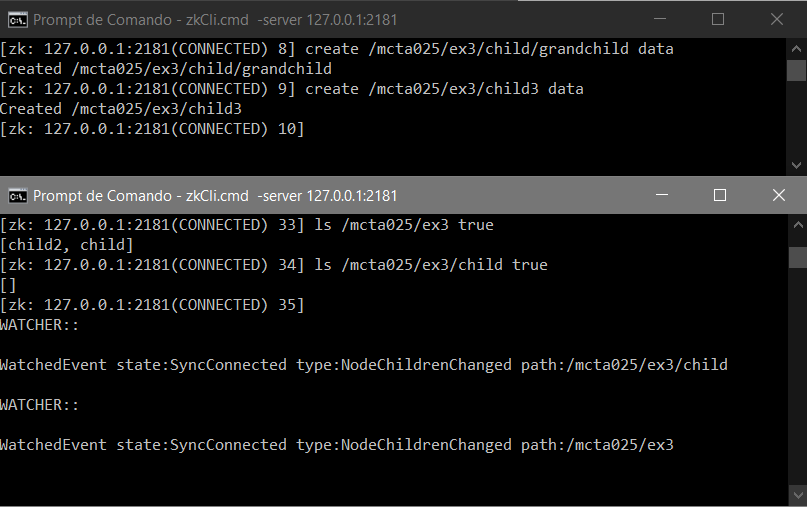
\includegraphics{pratica3/prints/roteiro 3.8.PNG}

\subsubsection{3.9 - Crie um watch de dados de um filho de /mcta025/ex3 e um watch de filhos para /mcta025/ex3 no Cliente 1. No Cliente 2, remova esse nó filho de /mcta025/ex3. O que aconteceu?}
\addcontentsline{toc}{subsection}{3.9 ?}

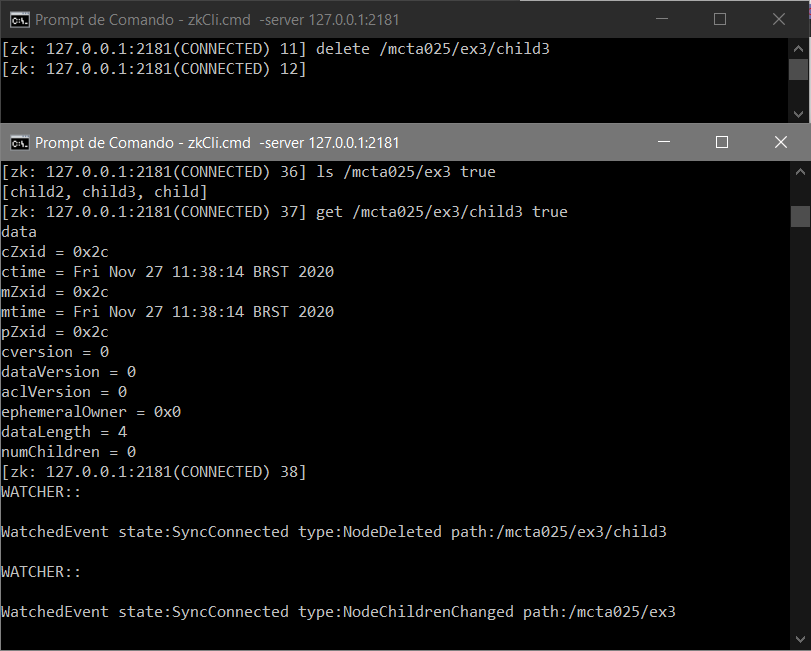
\includegraphics{pratica3/prints/roteiro 3.9.PNG}

\subsection*{4. ZooKeeper Java Example}
\addcontentsline{toc}{section}{4. ZooKeeper Java Example}


\subsubsection{4.1 - Execute o run.sh depois de acertar o valor da variável ZK para o diretório de instalação do ZooKeeper em seu computador.}
\addcontentsline{toc}{subsection}{4.1 ?}
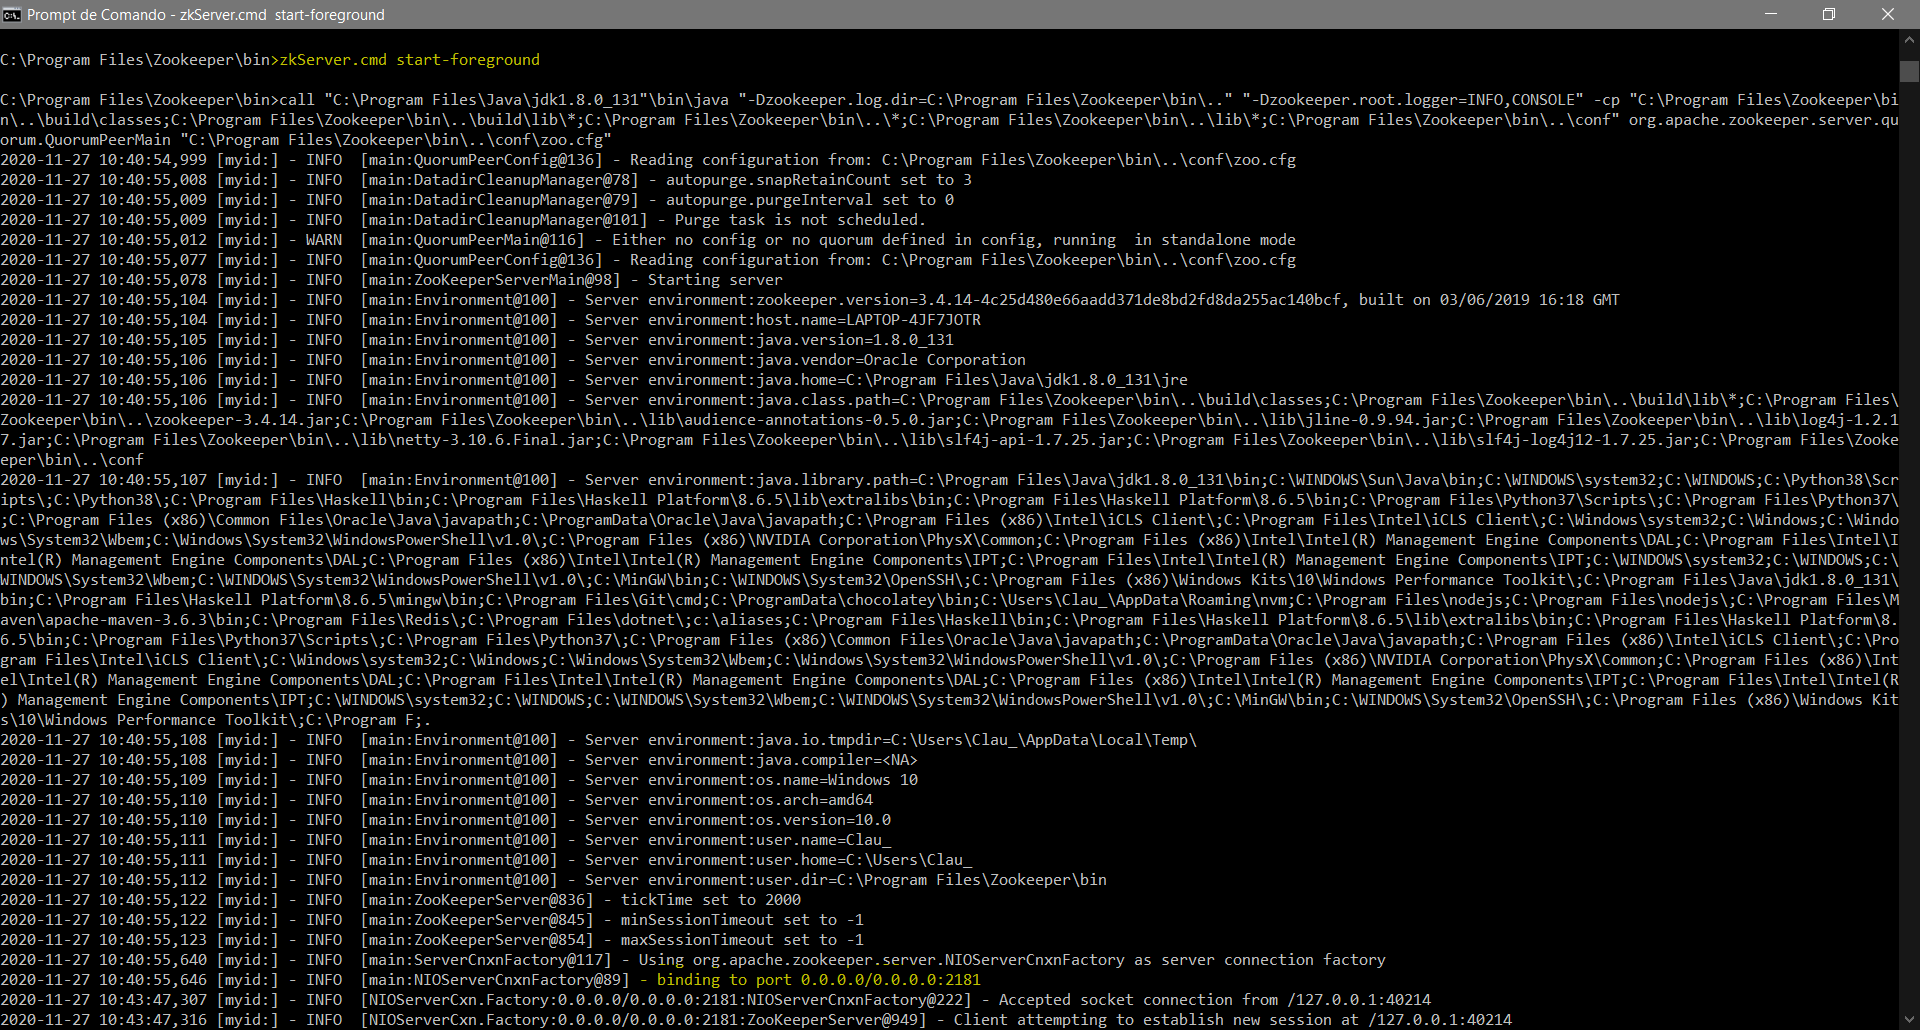
\includegraphics[width=20cm]{pratica3/prints/server_started.PNG}

\subsubsection{4.2 - Em uma CLI, crie um znode: create /mcta025/ex4 aData. O que
aconteceu?}
\addcontentsline{toc}{subsection}{4.2 Em uma CLI, crie um znode}

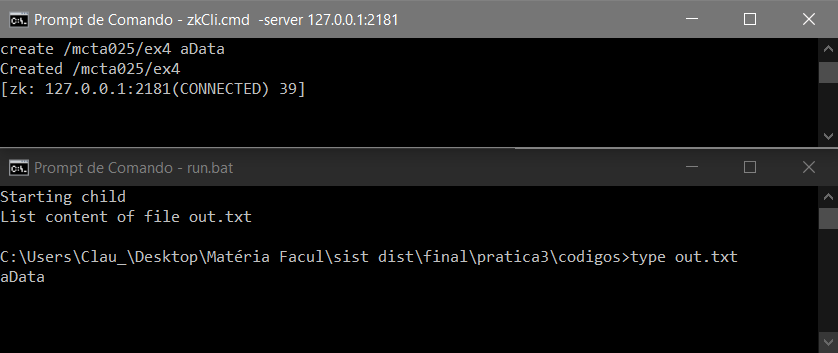
\includegraphics{pratica3/prints/roteiro 4.2.PNG}

\subsubsection{4.3 - Depois, mude o valor do nó: set /mcta025/ex4 newData. O que
aconteceu?}
\addcontentsline{toc}{subsection}{4.3 Depois, mude o valor do nó}
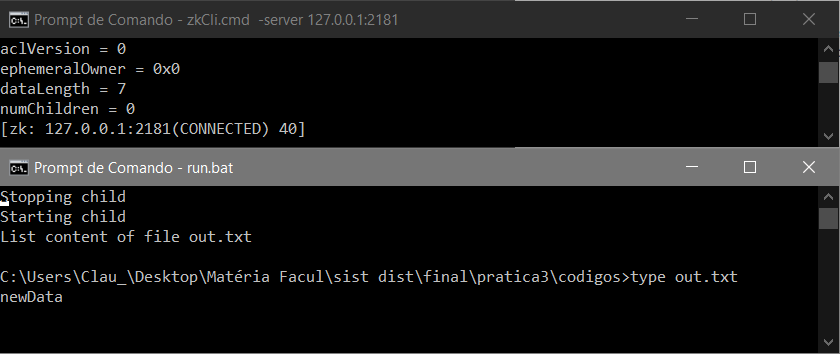
\includegraphics{pratica3/prints/roteiro 4.3.PNG}

\subsubsection{4.4 - Delete o nó: delete /mcta025/ex4. O que aconteceu?}
\addcontentsline{toc}{subsection}{4.4 Delete o nó}
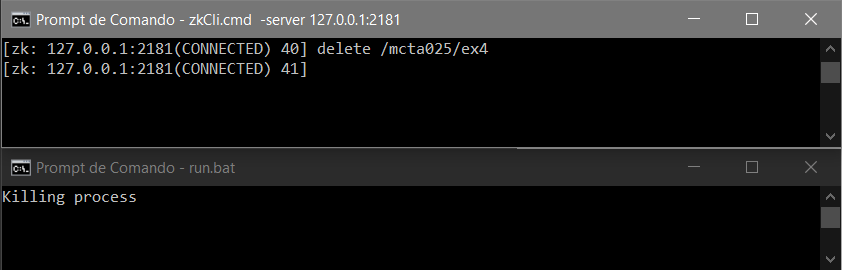
\includegraphics{pratica3/prints/roteiro 4.4.PNG}
